\paragraph{IUE02 Capturar movimientos} \hspace{1cm}\\ 
\label{pant:IUE02} 

\textbf{\textcolor[rgb]{0, 0, 0.545098}{Objetivo}}\\
Esta pantalla permite al Entrenador capturar un movimiento de técnica en la herramienta.\\

\textbf{\textcolor[rgb]{0, 0, 0.545098}{Diseño}}\\
La figura \ref{fig:IUE02} muestra el esqueleto del Entrenador en la parte central de la pantalla que sirve para realizar el seguimiento de su cuerpo.\\

La captura del movimiento comienza con una posición de inicio que depende del movimiento que se quiera capturar y la finalización depende de una posición final. Al término de la captura se guardara automáticamente el movimiento en la base de datos.\\

Para regresar a la pantalla anterior se debe realizar el gesto \textit{Regresar} para cancelar la captura y regresar a la pantalla IUE01 Menú Entrenador.

\begin{figure}[H]
	\centering
		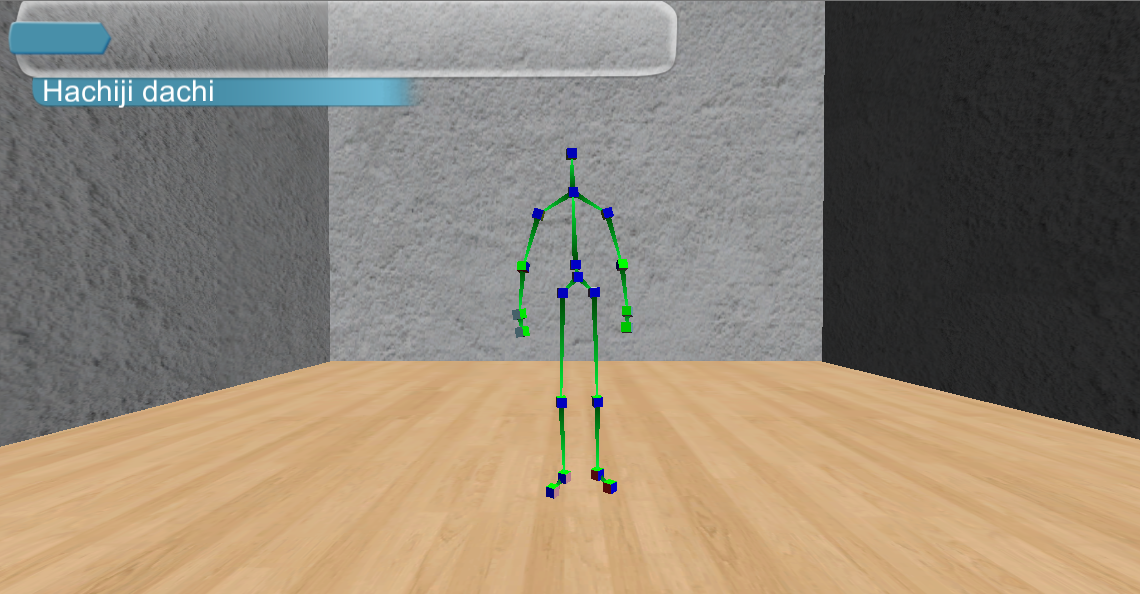
\includegraphics[scale=0.5]{./Figuras/Pantallas/IUE02Capturar_movimientos}
	\caption{IUE02 Capturar movimientos}
	\label{fig:IUE02}
\end{figure}

\textbf{\textcolor[rgb]{0, 0, 0.545098}{Entradas}}\\
En esta pantalla el Entrenador deberá capturar la siguiente información:

\begin{itemize}
	\item Movimientos de técnica por medio del sensor Kinect.
\end{itemize}
\vspace{1em}

\textbf{\textcolor[rgb]{0, 0, 0.545098}{Comandos}}
\begin{itemize}
	\item \textbf{\textcolor[rgb]{0, 0, 0.545098}{Comenzar captura:}} Permite al Entrenador iniciar la captura de un movimiento.
	\item \textbf{\textcolor[rgb]{0, 0, 0.545098}{Finalizar captura:}} Permite al Entrenador finalizar la captura de un movimiento.
	\item \textbf{\textcolor[rgb]{0, 0, 0.545098}{Regresar:}} Descarta los cambios y regresa a al menú de la pantalla \nameref{pant:IUE02}.
\end{itemize}

\vspace{1em}

\textbf{\textcolor[rgb]{0, 0, 0.545098}{Mensajes}}\\
	
\textbf{\nameref{msj:MSG01}}: Se muestra en la pantalla \nameref{pant:IUE02} cuando el Entrenador haya registrado al Practicante en la herramienta de manera exitosa.\\

\textbf{\nameref{msj:MSG25}}: Se muestra en la pantalla \nameref{pant:IUE02} cuando no se pueda guardar el movimiento en la base de datos.\\

\clearpage